\subsection{Shielding}

\subsubsection{Electromagnetic shielding mechanisms}\label{sec:irt_waves}

The following section outlines the fundamental theory of electromagnetic shielding. Throughout this thesis, all materials are assumed to be linear and isotropic.

A commonly used figure of merit for quantifying the shielding capability of a material is the electromagnetic shielding effectiveness $SE$. It is defined as the ratio of the incident to the transmitted electric field amplitude, expressed on a logarithmic scale in decibels as in \cites{10518640}[p.~63]{Jaroszewski_Thomas_Rane_2019}
\begin{equation}
	SE_{\mathrm{dB}} = 20\log_{10}{\left(\frac{E_\mathrm{i}}{E_\mathrm{t}}\right)},
	\label{eqn:se_elec_fields}
\end{equation}
where $E_\mathrm{i}$ and $E_\mathrm{t}$ denote the magnitudes of the incident and transmitted electric field, respectively, as shown in \autoref{fig:shielding_material_diagram}. An analogous expression holds for the magnetic field components. Higher values of $SE_{\mathrm{dB}}$ indicate greater attenuation of the electromagnetic field.

\begin{figure}[h]
    \centering
    \includegraphics[width=0.35\linewidth]{content/img/shielding_material_diagram.png}
    \caption{Incident, reflected and transmitted electric field intensities at a shielding material.}
    \label{fig:shielding_material_diagram}
\end{figure}

% (Note: Higher order modes may be able to propagate in the TEM cell, as the refraction of the shielding material follows to excitation of these modes.)

An electromagnetic wave incident on a shielding material may be partially reflected at the surface, partially absorbed within the material, and reflected multiple times internally before the remainder is transmitted. The total shielding effectiveness is determined by \cite[p.~63]{Jaroszewski_Thomas_Rane_2019}

\begin{equation}
	SE_{\mathrm{dB}}=R_{\mathrm{dB}}+A_{\mathrm{dB}}+B_{\mathrm{dB}},
	\label{eqn:se_rereflections}
\end{equation}


according to Schelkunoff's approach to shielding \cite{Schelkunoff_1938}. Absorption losses $A_{\mathrm{dB}}$ arise from waves propagating through the shield, $R_{\mathrm{dB}}$ denotes reflections at the material’s surface, and $B_{\mathrm{dB}}$ is a correction factor that accounts for multiple reflections within the shield \cite{10518640}.

Reflections contribute most significantly to a material’s shielding effectiveness \cite[p.~1]{Jaroszewski_Thomas_Rane_2019}. They are characterized by the reflection coefficient $R$. For a material to reflect incident fields, it must possess free charge carriers. For this reason, highly conductive materials, such as metals, reflect the majority of incident electromagnetic waves.

Reflections are caused by wave impedance mismatch between two materials. It is common practice to use the normalized wave impedance $Z$ to free-space wave impedance $Z_0$ when determining the reflection coefficient $R$. At the interface between free space and a shielding material, this yields \cite[p.~183]{Collin_2015}

\begin{equation}
	R=\frac{Z-1}{Z+1}.
	\label{eqn:reflection_coefficient_plane_dielectric}
\end{equation}

The normalized wave impedance is given by

\begin{equation}
Z=\frac{1}{Z_0}\sqrt{\frac{j\omega\mu}{\sigma+j\omega\epsilon}}.
\label{eqn:rel_wave_imp}
\end{equation}

Electric fields dominate in the near-field region of electric dipoles, as discussed in \cref{sec:ele_dip} and demonstrated with \eqref{eqn:compl_power_inf_elec_dipole}. Consequently, the wave impedance in this region is very high. For effective shielding by reflection, the shielding material should possess high permittivity and high conductivity to achieve a low impedance (see \autoref{eqn:rel_wave_imp}), creating the necessary impedance mismatch for reflection \cite[p.~67]{Jaroszewski_Thomas_Rane_2019}.

In contrast, magnetic fields are predominant in the near-field region of magnetic dipoles, as demonstrated with \cref{sec:mag_dip}, specifically with \eqref{eqn:pr_loop}. A high conductivity shields well against high-frequency magnetic fields due to creation of counter-acting eddy currents \cite[p.~112]{Jaroszewski_Thomas_Rane_2019}. Low-frequency magnetic fields are difficult to shield, and the most common approach is the redirection of magnetic flux lines due to high permeability of the shielding material \cite[pp.~112-113]{Jaroszewski_Thomas_Rane_2019}.

The portion of the electromagnetic wave that is not reflected is subject to absorption within the shielding material. This phenomenon is described by $A_{\mathrm{dB}}$ and accounts for an exponentially decreasing amplitude of an electromagnetic wave in a lossy medium. In conductive materials, this phenomenon is closely related to the skin depth.

The skin effect describes the interaction of electromagnetic waves with conductors, causing eddy currents to form on the surface. To investigate this phenomenon, the complex wavenumber is introduced $\tilde{k}=k + j\kappa$, which assists in mathematically describing waves propagating in lossy materials. The imaginary part $\kappa$ is expressed as

\begin{equation}
	\kappa = \omega \sqrt{\frac{\epsilon \mu}{2}}\left[\sqrt{ 1+\left(\frac{\sigma}{\epsilon\omega}\right) ^2 } -1\right]^{1/2}.
	\label{eqn:kappa}
\end{equation}

The skin depth $d$ is described by 

\begin{equation}
	d = 1/\kappa.
	\label{eqn:skin_depth}
\end{equation}

For highly conductive materials $\left(\sigma \gg \epsilon\omega\right)$ the skin depth is $d \propto 1/\sqrt{\omega}$. Therefore, high-frequency electromagnetic waves do not penetrate deeply into conductive materials, due to the free electrons associated with high conductivity absorbing the waves with eddy currents on the material's surface and transforming the energy into heat. A material's permeability further reduces the skin depth due to the increased susceptibility to eddy currents \cite[p. 104]{Jaroszewski_Thomas_Rane_2019}.

For non-conductive materials, absorption depends on the electric loss factor \cite[pp.~102-103]{Jaroszewski_Thomas_Rane_2019}, as further described in \cref{sec:shielding_parameters}.

Upon reaching the far end of the shielding material, re-reflections can occur. When the material thickness is greater than the skin depth, the correction factor for this effect $B_{\mathrm{dB}}$ can be neglected. When the material thickness is smaller than the skin depth, however, the internal reflections reduce the shielding effectiveness by destructively interfering with the reflected waves, and the value of $B_{\mathrm{dB}}$ is negative \cite[p.~1]{Jaroszewski_Thomas_Rane_2019}.

%Conductor losses $P_\mathrm{loss}$ are linearly proportional to the area of the conductor and therefore the Skin depth. They show the same dependency on the frequency $P_\mathrm{loss}\propto 1/\sqrt{\omega}$ \cite[p. 413]{Griffiths_2024}. 

\subsubsection{Conductivity, permeability and permittivity in shields}\label{sec:shielding_parameters}

%The reflection coefficient can be converted into dB, leading to $R_\mathrm{dB}$. Any additional reflection happen due to re-reflections inside the shielding material, described by $B_\mathrm{dB}$. The rest of the energy must either be absorbed, described by $A_\mathrm{dB}$ or transmitted, shown by $T_\mathrm{dB}$. 

%\todo{p. 309 Classical Electrodynamics (John David Jackson) describe shielding material by dipole moments}


%The wavenumber $k$ in lossy media consists of a real and an imaginary, parts as in
%
%\begin{equation}
%	k = \beta + \mathrm{i}\alpha.
%	\label{eqn:wave_number}
%\end{equation}

%The imaginary part of the wavenumber $k$, $\alpha$ denotes the attenuation or absorption coefficient. It describes the reduction of the intensity of the wave over distance.

When molecules in a material are exposed to an electric field, they become polarized. This property is characterized by the material's permittivity $\epsilon$. Exposure to a magnetic field causes the spins of electrons within atoms to align with the field, described by the material’s permeability $\mu$. When these electric and magnetic fields vary with time, the molecules continuously move and realign, resulting in the movement of charges, which is quantified by the conductivity $\sigma$. The energy lost in this dynamic process is dissipated as heat \cite[p.~68]{Balanis_2012}.

The electric field pushes charges in polarizable molecules apart. This separation of charges may be described as an electric dipole, depending on the separation distance and the charge. Under alternating electric fields, the movement of charges contributes to $\sigma$. This phenomenon is called dielectric hysteresis. It is quantified by the loss tangent $\tan\delta_e$, and defined as \cite[pp.~73-74]{Balanis_2012}

\begin{equation}
	\tan\delta_e = \frac{\sigma_s}{\omega\epsilon'}+\frac{\epsilon''}{\epsilon'}.
	\label{eqn:loss_tangent_permittivity}
\end{equation}

There, $\sigma_s$ is the static conductivity, indicating the conductivity of the material for constant fields over time. The complex part of the permittivity $\epsilon''$ describes the lossy part of the dielectric material, specifically relevant for alternating fields over time. The real part of the permittivity is lossless and is noted by $\epsilon'$, and corresponds to the material's ability to store electric energy \cite{Kruželák_Kvasničáková_Džuganová_Dosoudil_Hudec_Krump_2024}. The overall complex permittivity is therefore $\epsilon=\epsilon'+j\epsilon''$.

The loss tangent therefore relates the conductivity of a material to the real permittivity. A dielectric with low losses has a much larger displacement current than conduction current density ($\tan\delta_e \ll 1$). The opposite is true for a good conductor ($\tan\delta_e \gg 1$) \cite{Balanis_2012}.

%The loss tangent $\tan\delta_e$ is a function of frequency, however, it is often not stated as such. Therefore, the loss tangent of FR4, for example, is given as $\tan\delta_e=0.02$ for frequencies up to 1\,GHz. For higher frequencies, the molecules may have resonance frequencies, where they influence more strongly the overall conductance and consequently increase the imaginary part of the permittivity $\epsilon''$.

Analogous to polarizable materials, there are also magnetizable lossy materials, which are characterized by a complex permeability $\mu=\mu'+j\mu''$. The real part of the permeability $\mu'$ describes the material's ability to store magnetic energy, while $\mu''$ describes the magnetic losses  \cite{Kruželák_Kvasničáková_Džuganová_Dosoudil_Hudec_Krump_2024}. The complex permeability can also be described by a magnetic loss tangent $\tan{\delta_m}$, as shown in

\begin{equation}
	\tan{\delta_m}=\frac{\mu''}{\mu'}.
	\label{eqn:magnetic_loss_tangent}
\end{equation}

The loss tangent is very low for the majority of materials. Ferrites are a notable exception and are commonly used to attenuate high-frequency signals \cite[p.~80]{Balanis_2012}.

\subsubsection{ASTM ES7-83 Method}\label{sec:astm}

The ASTM ES7-83 method is used to determine the shielding effectiveness of shielding materials in far-field conditions. The shielding material is inserted into a coaxial TEM cell around the septum. Ideally, they form a continuous connection \cite{MORARI_BĂLAN_2015}. 

In this method, two measurements are performed at the output ports of the TEM cell. In the first measurement, an empty TEM cell is excited and a reference output voltage $U_\mathrm{ref}$ is measured. In the second, the TEM cell is loaded with the shielding material, and the output voltage $U_\mathrm{load}$ is again noted. The shielding effectiveness $SE_\mathrm{dB}$ is then derived with the obtained measurement values by \cite{MORARI_BĂLAN_2015}


\begin{equation}
	SE_\mathrm{dB}=20\cdot\log{\left(\frac{U_\mathrm{ref}}{U_\mathrm{load}}\right)}.
	\label{eqn:SE_voltages}
\end{equation}

When applying numerical analysis in combination with this method, it is more convenient to define a reference output power $P_\mathrm{ref}$ for an unloaded TEM cell, and an output power for the loaded case $P_\mathrm{load}$. This leads to similar expression, 

\begin{equation}
	SE_\mathrm{dB}=10\cdot\log{\left( \frac{P_\mathrm{ref}}{P_\mathrm{load}} \right)}.
	\label{eqn:SE_power}
\end{equation}

\autoref{fig:form_of_shielding_material} shows the cross section of this shielding material, which is inserted into the TEM cell. In \autoref{fig:ASTM ES7-83} the shielding material can be seen wrapped around the septum. 

\begin{figure}[h]
    \centering
    \begin{subfigure}[h]{0.49\textwidth}
        \centering
        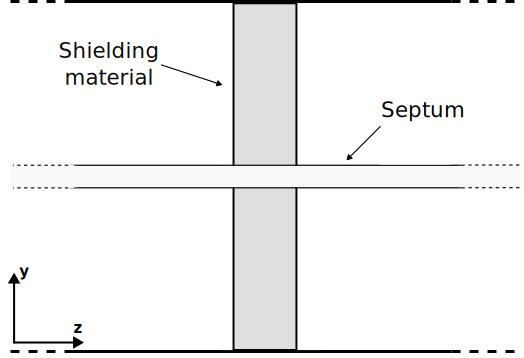
\includegraphics[width=\textwidth]{content/img/ASTM ES7-83.png}
        \caption{$yz$-plane}
        \label{fig:ASTM ES7-83}
    \end{subfigure}%
    \hfill
    \begin{subfigure}[h]{0.49\textwidth}
        \centering
        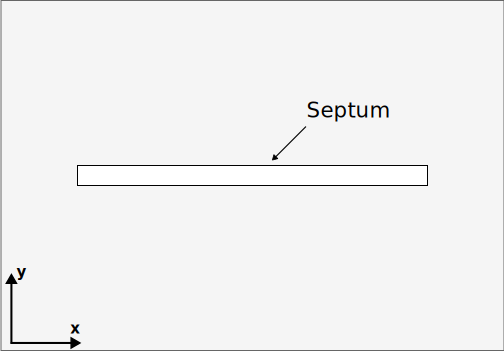
\includegraphics[width=\textwidth]{content/img/form_of_shielding_material.png}
        \caption{$xy$-plane}
        \label{fig:form_of_shielding_material}
    \end{subfigure}
    \caption{Cross section of shielding material in TEM cell}
    \label{fig:subfigures}
\end{figure}

Then, the S-parameters derived in the simulations are used to determine the output powers $P_\mathrm{ref}$ and $P_\mathrm{load}$. By exciting the TEM cell with a power of 1\,W, the reference power $P_\mathrm{ref}=1\,\mathrm{W}$. The measured power is then derived through

\begin{equation}
    P_\mathrm{load}=P_\mathrm{ref}\cdot10^{S_\mathrm{12, dB}/10}.
    \label{eqn:load_power}
\end{equation}

\subsubsection{Dual TEM cell}\label{sec:dual_tem_cell}

The shielding effectiveness of a material may also be determined using a dual TEM cell shown in \autoref{fig:dual_tem_cell}. The two cells are connected through an aperture, which can be filled with the shielding material or left empty. The upper TEM cell is excited through port 1, and acts as a driving cell, transmitting power through the aperture. Port 2 is loaded with the reference impedance $Z_w\approx50\,\Omega$. The second TEM cell functions as a receiver, collecting power at its output ports \cite{MORARI_BĂLAN_2015}.

\begin{figure}[h]
	\centering
	\includegraphics[width=0.75\linewidth]{content/img/dual_tem_cell.png}
	\caption{Dual TEM cell with aperture}
	\label{fig:dual_tem_cell}
\end{figure}

If the aperture is electrically small, its coupling may be described by an electric and a magnetic dipole moment. Their magnitude is related to the electric and magnetic coupling between the TEM cells over the aperture. Therefore, the electric and magnetic coupling can be determined separately by adding or subtracting the output powers of the receiving TEM cell \cite{MORARI_BĂLAN_2015, 4091811}. Consequently, an electric shielding effectiveness $SE_\mathrm{dB}^\mathrm{e}$ and a magnetic shielding effectiveness $SE_\mathrm{dB}^\mathrm{m}$ can be calculated with

\begin{subequations}
	\begin{equation}
		SE_\mathrm{dB}^\mathrm{e}=10\log{\left( \frac{P_\mathrm{ref, sum}}{P_\mathrm{load,sum}} \right)},
		\label{eqn:se_dual_cell_e}
	\end{equation}
	\begin{equation}
		SE_\mathrm{dB}^\mathrm{m}=10\log{\left( \frac{P_\mathrm{ref, diff}}{P_\mathrm{load,diff}} \right)}.
		\label{eqn:se_dual_cell_m}
	\end{equation}
\end{subequations}

Separating the electric and magnetic shielding effectiveness is useful when applying shielding materials in the near field of electric or magnetic dipole moments. For shielding a magnetic dipole moment, the $SE_\mathrm{dB}^\mathrm{m}$ value is considered significant \cite{4091811}, whereas for an electric dipole moment, the $SE_\mathrm{dB}^\mathrm{e}$ value is relevant.

%Because the normalized electric field at the aperture will be of TEM mode, only the component normal to the aperture in z-direction has to be considered. Just as in the case of dipole representation, the Lorentz Reciprocity theorem may be applied to find the fields in the TEM cell. Because both the fields at the output and in the aperture are of TEM mode, only the E-field at the output may be considered. 



